\documentclass[12pt,a4paper]{scrartcl}

%%%%%%%%%%%%%%%%%%%%%%%%%%%%%%%%%%%%%%%%%%%%%%%%%%%%%%%%%
% Validation Report                                     %
% Proof Searching and Proof checking                    %
% Computing Group Project 2010                          %
%%%%%%%%%%%%%%%%%%%%%%%%%%%%%%%%%%%%%%%%%%%%%%%%%%%%%%%%%

% standard packages
\usepackage[latin1]{inputenc}
\usepackage{amssymb, amsmath, amsthm}
\usepackage{fancyhdr}
\usepackage{graphicx}
\usepackage{longtable}
\usepackage{appendix}

% for the code listings (if any)
\usepackage{listings}
\lstset{language=Haskell, numbers=left, 
  showstringspaces=false, frame=single}

% for harvard-style citation
\usepackage{natbib}

% double spacing
\usepackage{setspace}
\doublespacing

\begin{document}

% the first page
\thispagestyle{empty}
\begin{titlepage}
  \begin{center}
    \vspace*{\fill}
            {{\Large Imperial College London\\ Department of Computing\\}}
            \vfill {{\Huge Proof Searching \& Proof Checking \\
                \vspace{0.2cm}
                     Final Report}}\\
            \vfill {{\large Computing Group Project\\ 
                Supervisor: Dirk Pattinson\\ Autumn 2010}}
            \vfill {Jannis Bulian, jb1508@ic.ac.uk, 567339 \\
                    Michal Parusinski, mgp08@ic.ac.uk, 566542 \\
                    Ka Wai Cheng, kwc108@ic.ac.uk, 548464\\
                    Saguy Benaim, ssb08@ic.ac.uk, 552374}
  \end{center}
\end{titlepage}

\newpage

\tableofcontents
\thispagestyle{empty}

\newpage

\section{Introduction}
This report is the final report for the Proof Search meets Proof Check
project, which is about formal reasoning in Description Logic a
knowledge representation language.  More specifically our project is
about deciding the satisfiability or otherwise unsatisfiability of a
set of concepts with a given knowledge base by generating a model (for
satisfiability) or otherwise a proof (for unsatisfiability), and
checking automatically the outputs for correctness. The report will
provide a detailled account of most aspects involved in the project.

After introducing to our project we will first explain the theoretical
and technical background involved in the project, then we will mention
all engineering aspects of the project both managerial and
technical. Amongst the engineering aspects we will comment upon are
our Software Development practices, our testing pratices,our progress
of the project and the use of the technology available. Finally we
will end with an asssessement on the success of the project.


\section{Overview (high level description)}

The main goal of our project was to create a tool for formal reasoning
in a knowledge representation framework called Description Logic. More specifically a solver for Description Logic. Description Logic find
many uses in Artificial Intelligence, Bioinformatics and Web
Semantic. The latter is one of the most prominent examples of
application of Description Logic since it provides a way create a
knowledge domain for websites, and hence has potential to improve
the ``surfing on the web'' experience.

More specifically our software provides a tool for showing
satisfiability or otherwise unsatisfiability in Description Logic by
generating a model (for satisfiability) or a proof (otherwise). The
program was written in Haskell for the GHC (Glasgow Haskell Compiler)
Platform and is intented to run on most platforms. It has been tested
on Windows, Mac OS X and Linux and is licensed under the open-source
license GPL 3.0.

Unlike most other Description Logic solvers which are focused on Web Semantics
 our software is targeted for academia: it is highly flexible
especially since the software has been written in the high level
pratical for logic language Haskell and is open-source; also it
focuses on providing short, correct and clear output of the obtained
models and proofs in a graphical or a textual format, thus the
software can help study the theory of Description Logic.



\section{Technical background \& description}
Our project is focused on reasoning in Description Logic a language
for representing knowlegde.  We will provide a short but technical
definition of what we mean by Description Logic. The logical framework
the software deals with is formally known as $\mathcal{ALC}$
(\textit{Attributive Concept Language with Complements}). It forms the
basis for many other Description Logics, and it can be seen as a more
expressive extension of Propositional Logic and a decidable subset of
First-Order logic.

Like in other logics $\mathcal{ALC}$'s definition is subdivided in two
parts one syntactic (language) and the other semantic (meaning). The
syntax is built upon two sets: A set of atomic concept names (unary
relations) and a set of relation names (binary relations). Those two
sets defines the signature. A signature for instance could be
consisting of the following atoms: ``Book'', ``Film''; and the
following relations: ``Bought'', ``Borrowed''. We will now define what
a concept is. A concept in Description Logic is a statement of truth
and falsity just like formulaes are statements of truth in First-Order
logic.

Anything of the following form is a concept:
\begin{itemize}
\item $\top$ (``truth'', ``tautology''),$\bot$ (``bottom'', ``falsity'') and any atomic concept name $A$ is a concept.
\item If $C$ and $D$ are concepts then $C \sqcap D$ is a concept
  called the intersection (or the conjunction) of $C$ and $D$.
\item If $C$ and $D$ are concepts then $C \sqcup D$ is a concept
  called the union (or the disjunction) of $C$ and $D$.
\item If $C$ is a concept then $\neg C$ is a concept called the complement (or the
  negation) of $C$.
\item If $C$ is a concept and $R$ a relation name then $\forall R . C$
  and $\exists R . C$ is a concept called each respectively the
  universal and existential restriction of $C$.
\end{itemize}

Nothing else is a concept. Examples of concepts are $\forall Link
. (Website)$ or $\exists Friend . (\neg Facebook)$. The 
formal semantic for $\mathcal{ALC}$ is defined the notion of
interpretation which gives meaning for Description Logic concepts. An
interpretation is a pair $(\Delta^{I},.^{I})$, where $\Delta^{I}$ is a
non-empty set called the domain and $.^{I}$ is a function sending each
atomic concept to a subset of $\Delta^{I}$ and each relation name to a
subset of $\Delta^{I} \times \Delta^{I}$ and satisfying the following 
properties:

\begin{itemize}
\item $\top^{I} = \Delta^{I}$ and $\bot^{I} = \emptyset$.
\item $(C \sqcap D)^{I} = C^{I} \cap D^{I}$.
\item $(C \sqcup D)^{I} = C^{I} \cup D^{I}$.
\item $(\neg C)^{I} = \Delta^{I} \backslash C^{I}$.
\item $(\forall R . C)^{I} = \{x \in \Delta^{I} \text{: forall } (x,y) \in R^{I} \text{ implies } y \in C^{I}\}$ 
\item $(\exists R . C)^{I} = \{x \in \Delta^{I} \text{: exists } (x,y) \in R^{I} \text{ implies } y \in C^{I}\}$ 
\end{itemize}

We sometimes say that a specific intrepretation is a model. 

An intuitive way to think about $\mathcal{ALC}$, is that we are given
a set of properties an individual might satisfy or not and a set of
possible relations between them. Description Logic in $\mathcal{ALC}$
provides a way to give a representation of knowledge about the
individuals, properties and relations.  $\top$ and $\bot$ are
statements that are either always true or respectively always false
for each individual.  $\sqcap$, $\sqcup$ and $\neg$ can be read each
as ``and'', ``or'' and ``not''. $\forall$ and $\exists$ differs a bit
from First-Order logic in the sense $\forall R$ means every
``R-successors'' and $\exists R$ means a ``R-successors''. For
instance $\forall Link . Website$ could be read as ``every link is to
a website'' and $\exists Friend . (\neg Facebook)$ could be read as
``some friend is not on facebook''

A knowledge base in Description Logic is defined by two collections of
concepts for some signature in $\mathcal{ALC}$. The first one are the
global assumptions often written as $\gamma$ and we will refer here
as \textit{Gamma} and the second one are the initial set of concepts
which we will refer here as the \textit{Givens}. We say a knowledge
base is satisfiable if there exists an interpretation or model that
makes every statement in \textit{Gamma} true at each point of
$\Delta^{I}$ and every statement in \textit{Givens} true at some point
in $\Delta^{I}$. If no such model exists we say a knowledge base is
unsatisfiable. For example if \textit{Givens} consists of one concept
namely $\exists R. \top$ and if \textit{Gamma} consists of also one
concept only $A$ (an atomic concept name), then this knowledge base is
satisfiable since the intrepretation $\Delta^{I} = \{1\}$ with $A^{I}
= \{1\}$ and $R^{I} = \{(1,1)\}$ is a model. In other words a concept
in \textit{Gamma} is satisfied if its interpretation is $\Delta^{I}$,
and a concept in \texit{Givens} is satisfied it its interpretation is
a non-empty subset of $\Delta^{I}$. If some global assumptions together
with an initial set of concepts is unsatisfiable, i.e. no model exists 
then we can show unsatisfiability through a proof. 

\subsection{Tableaux Calculus}

Our goal is to produce a model if we can. If we are not able to produce
a model, we want to give an argument, a proof, why this is not possible.
Consider for example the relation \emph{Eat} interpreted as
\[
aEatb \iff \text{a eats b}.
\]
Say we have the following requirement for a pizza: It should be vegetarian
and with salami. This is surely not satisfiable. We want a proof theory
that gives us the same result.

Formally, we use the \emph{Tableaux Calculus} as defined in \cite{gore07}. In the
following $A, B$ usually stand for atoms, while $C,D$ denote concepts. Suppose
we have a set of global assumptions $\Gamma$ and a set of givens $X$. We define
a set of rules, consisting of an `upper' side with the givens, and a `lower' side
with the consequences $Y_i$ as in
\[
(\text{rule}) \, \Gamma: \frac{X}{Y_1 | \dots | Y_k}.
\]
The `denominator' can be seen as the result of a reasoning progress that goes downwards,
i.e. if $X$ is satisfiable, then one of the $Y_i$ is also satisfiable. We define the
following rules:
\[
(\bot) \, \Gamma: \frac{X; A; \lnot A}{\bot}, \quad
(\sqcap) \, \Gamma: \frac{X; C \sqcap D}{X; C; D}, \quad
(\sqcup) \, \Gamma: \frac{X; C \sqcup D}{X; C | X; D},
\]
\[
(\exists R) \, \Gamma: \frac{X; \exists R. C}{\{D | \forall R.D \in X\};  C ; \Gamma}.
\]
Intuitively this means, we can derive falsity from a contradiction ($\bot$), we derive
$C$ and $D$ from knowing that both are true ($\sqcap$), we can derive either $C$ or $D$
from knowing that one of them is true ($\sqcup$). The last rule is a bit more complicated, it
means that whenever we know that there is an $R$-successor that satisfies C, it must
also satisfy $\Gamma$ (because that's true everywhere) and all the things that have
to be true at an $R$-successor, i.e. $\{D | \forall R.D \in X\}$.

Starting with a root with $X$ and $\Gamma$ this gives a tree structure, called a tableaux.
We call a branch closed if the last child is $\bot$ and a tableaux closed if all the
branches are closed. Otherwise, we call the tableaux open. Given a set of global
assumptions $\Gamma$, a set of concepts $X$ is unsatisfiable if and only if there
is a closed tableaux from $\Gamma; X$. We call this a proof. This proof calculus
is sound and complete with respect to $\mathcal{ALC}$. (See e.g. \cite{gore07} for a
proof.)

We can now make a formal argument for the example above. Say we have no global
assumptions, and the two statements $Vegetarian$ and
$\lnot Vegetarian$. We get the simple proof
\[
(\bot) \frac{Vegetarian; \lnot Vegetarian}{\bot}.
\]

We now have the theoretical means to say whether a certain concept is satisfiable
or not. Our program will automate this for us.

\subsection{Description of Main Components}

Our program makes use of the theory presented above to say whether a given concept
is satisfiable or not (assuming some global knowledge). To make sure this is correct
(and convince skeptical users) the program will provide either a model or a proof.
The main components are illustrated in Figure~\ref{components}. A \emph{parser} translates
the user input into an internal language that is processed by the
\emph{proof/model searcher}.
In case a model is found, we say it is satisfiable and provide a model that can be
checked by the \emph{model checker}. Otherwise we give a proof that can be checked
by the \emph{proof checker}.

\begin{figure}
  \caption{The main components of the program.}
  \begin{center}
    \includegraphics[scale=0.4]{design.jpeg}
  \end{center}
  \label{components}
\end{figure}

\paragraph{Parser.}

The purpose of the parser is to read the input from the user
and transform it into a format that can be used by the rest of the program. We have
written three different lexers that interpret
\begin{itemize}
\item the user input from the command line (lexerI),
\item modal formulas from the TANCS 2000 Problems\footnote{http://www.cs.man.ac.uk/~schmidt/mspass/problems.html} (lexerB1),
\item modal formulas from the logics work bench\footnote{http://iamwww.unibe.ch/~lwb/benchmarks/benchmarks.html} (lexerB2).
\end{itemize} 
The actual parser is automatically generated from a grammar we specified.

\paragraph{Proof/Model Searcher.} 

The proof/model searcher receives the knowledgebase and a set of concepts and returns
either a proof or a model. The implementation is similar to the one described in
\cite{gore07}, but additionally a proof and a model are simultaneously build, maintained,
and eventually one of them returned. It consists of the following components:
\begin{itemize}
\item \emph{findProofOrModel}: This is the `entrance' function that maintains
a cache and looks up the current set of concepts. If it is found, it returns the
found result. Otherwise, and certainly in the beginning, the function
\emph{findProofOrModel'} is called. This function expects the concepts to be in
a certain order, so this order is always maintained (using \emph{conceptSort}).

\item \emph{findProofOrModel'}: This function has a case for every possible concept. If no
contradiction is found and it is not done yet, it creates both a model and a proof
after recursively calling \emph{findProofOrModel} on the remainder. For the more
complicated
exists case it calls the function \emph{foldExists}. When it is done, and there was no
contradiction, it calls \emph{constructAtomicModel} to create a model.

\item \emph{foldExists}: It deals with all the exists formulas, by going through them
one by one and generating a proof or model with \emph{applyExists}
for each of them. If a proof is found for one of
the successors, this proof is immediately returned. If all the exists formulas
supplied models, they are joined using \emph{joinModels} and returned. Because
the function has to keep track of the individuals used in each model, we decided
to choose a `fold' approach with caching in favor of parallelism.
\end{itemize}
The result is either a proof or a model, which can be checked with the proof and
model checkers.


\paragraph{Proof Checker.}

The main purpose of the proof checker component of the program is to ensure the proof produced by the proof construction component is: correctly formed, independent of the implementation of the proof search; and proves unsatisfiability given the initial set of formulas and global assumptions. However, the proof checker will check any proof structure passed to it, including proofs that may be given by the user rather than produced by the proof construction component of our program.

 The proof checker is called by the function checkProof with the actual proof tree to check and the global assumptions that the proof was constructed against as expected inputs. The expected output of the proof checker is a tuple consisting of a String and a Boolean. The Boolean has the value True when each step in the proof applies a proof rule correctly in the tableau calculus described in the Background section; and shows unsatisfiability by closing with a contradiction or falsity in all branches of the proof. Otherwise, the Boolean returned has the value False and the String is a message detailing why the proof tree is incorrect or does not show unsatisfiability. Hence the string is empty if the proof tree is correct.

 The proof checker is made up of the following components:

\begin{itemize}
\item checkRule: function that, given a proof step (containing the set of concepts, rule to apply and the specific concept to apply the rule to) and global assumptions, returns a tuple (error message, True if the rule can be applied to the concept, list of expected results of applying the rule).

\item checkProofStep: function that checks a single proof step, returning the result of calling checkRule if the concept to apply the rule to is contained in the set of concepts at this step of the proof. Otherwise, a message that the concept does not exist and False are returned.

\item checkTree: function that checks the set of concepts at the next step is the same as the expected results, then if this is true, does a recursive call on the subtree of the proof. Otherwise, a message that the next step's set of concepts does not match the expected results of applying the rule to this step's set of concepts. For leaf nodes of the proof tree structure, checkTree checks that the rule applied closes the branch in the proof with a contradiction or falsity, hence showing unsatisfiability.

\item checkProof: function that is called by other modules to check the given proof with global assumptions is a valid proof (each proof rule is applied correctly and the proof shows unsatisfiability). Some initial checks are performed to ensure the concepts are all in negation normal form and the global assumptions are contained in the initial set of concepts at the root of the proof tree. If all checks pass, the result of calling checkTree with the same arguments is returned.
\end{itemize}

\paragraph{Model Checker.}
  The main purpose of the model checker component of the program is to
  ensure the model produced by the model construction component is:
   correctly formed, independent of the implementation of the proof/model
   search; and justifies satisfiability given the initial set of formulas
   and global assumptions. However, the model checker will check any
   model structure passed to it, including models that may be given by
   the user rather than produced by the model construction component of
   our program.

   The model checker is called by the function checkInputModel with the actual
   model, global assumptions and the initial set of formulas to check
   the correctness of the model. The expected output of the
   model checker is a tuple consisting of a String and a Boolean. The
   Boolean has the value True when the model is correct with respect
   to the global assumptions and the initial set of formulas, in other words
   each concept in the Global Assumption is true at each point and each concept  in the
   initial set of formulas is true at some point.
   Otherwise, the Boolean returned
   has the value False and the String is a message explaining which
   element fails to make the model correct.
   Hence the string is empty if the model is correct.

   The model checker is made up of the following components:

\begin{itemize}
\item checkInputModel: The most global function for the model checker.
   It calls two functions: checkGivens and checkGamma that checks that
   the global Assumptions and the initial set of concepts are satisfied
   in the model. It combine the result of both function which are tuples of
   the form described above. If one of the two functions returns false then
   the result if False with the corresponding a message telling why
   the model is invalid which is obtained by combining the two Strings
   obtained from checkGivens and checkGamma. Otherwise True with
   an empty String is returned.

\item checkGamma and checkGivens: Both function behave in a similar way,
   the functions use a subroutine called checkConcept, which checks if a concept is
   satisfied at a distinguished element of the domain. It performs that subroutine
   for each element of the domain. At each point we get a result of the form
   described as above: a tuple of a Boolean and a String. The results are
   then combined by using a function called answerAnd for checkGamma
   and answerOr for checkGivens. answerAnd stops as soon as one tuple
   of the form (False, message) is found and then returns that results, if no such
   tuple is found it returns (True, ""). answerOr stops as soon as a result of
   the form (True, "") is found otherwise it combines all the message (False, message)
   together by concatenating the messages.

\item checkConcept: It checks if a concept is true at a distinguished element. Its input is of a
   concept, a model, a distinguished element of the domain. It returns a tuple as described
   above. It returns (True,"") if the concept is satisfied at that point otherwise it tells what
   was wrong. The check is performed recursively until an atomic concept is obtained where it
   simply check if the distinguished element satisfied that concept in the model. And, Or and Negation
   are done in the intuitive way. For universal and existential restriction of the form (Forall R . C) or
   (Exists R . C) it checks if all successors or respectively some successors satisfies C using checkConcept again.
   The results are combined also using answerAnd and respectively answerOr.
\end{itemize}

To summarize the above, our main achievements are:
\begin{itemize}
\item representation of concepts, models and proofs from description logic,
\item implementation of a parser for reading concepts in description logic,
\item implementation of a model/proof searching algorithm for description logic which is correct and which terminates (with high confidence),
\item the implementation of a model checking algorithm for description logic that checks if a model is correct,
\item implementation of a proof checking algorithm for description logic that checks if a proof is correct,
\item a user interface to the program,
\item provision of a standard output format for generated models and proofs as well as a user-friendly graphical representation,
\item output of a helpful explanation in case a proof or model turns out to be incorrect.
\item provision of an interface to the model/proof checker that allows users to check their own proof model (i.e. independence of proof/model generation and checking).
\end{itemize}

\section{Software Engineering Issues}
\subsection{Technology Used}

We used several tools and languages in our program, with the main programming language being Haskell. Other than Haskell, the parser generator, Happy, was used to produce the Haskell code for the parser component of the program. For the output of models and proofs into more readable format, Graphviz and Latex were used respectively.

Haskell, was chosen as the main programming language primarily because Haskell's pattern matching naturally implements the handling of cases (such as proof rules and formulas) together with way we decided to structure the program into the main components. This way work on the different components can be implemented independently and simultaneously. Other reasons why Haskell was more appealing than other programming languages considered (Java, C, C++) were Haskell's compact code and each team member's relative levels of programming skills and experience in each language.

With no prior experience in programming a parser, we considered using Happy and Parsec in implementing the parser component for user input and benchmark files. Happy is an LR (bottom-up) parser generator and requires Happy to be run to generate the Haskell code for the parser, whilst Parsec is a LL (top-down) parser library for Haskell so does not require this pre-processing stage.

All members of our team have not used either of these before and so the decision to use Happy was based upon the available documentation. Happy's documentation was clearer and we observed that it involved simpler hand-written code. Hence, we believed the parser would be completed in a shorter amount of time by using Happy. The only disadvantage is that Happy needed to be run after any changes to the Happy file to generate, but this would only be required in the development stages and not when used by end users.

For the output of proofs, 

On the other hand, for the output of models, Graphviz was used. Graphviz is an open source graph visualisation software that have tools and libraries

\subsection{Technical Challenges}

We encountered a few technical challenges throughout the development of this project. The most problematic were the implementation of caching in the proof/model search component and in extending our program to allow users to express specific individuals that must exist and to reason with. These problems were addressed by our frequent informal meetings, in which we discussed the difficulties arisen and finding ways to resolve them.

In the early iterations, we discovered the potential problem of cycles in the input global assumptions, which causes complications in the implementation of proof search, model construction and model checking. To prevent the proof/model search component from potentially becoming non-terminating, we decided to implement a mechanism for caching the sets of concepts already expanded and their resulting proof or model.

Extending the already written proof/model search component to cover this was very challenging because proof construction and model construction are performed simultaneously in our implementation. By implementing caching, the code became much more complex than before and as a result, it was difficult to reason the correctness of code and to debug for very specific cases.

This issue was addressed in our frequent group meetings by discussion, using code reviews, and bug tracking system. In this way, other members of the group not assigned to the implementation of the proof/model search aided in locating and fixing bugs.

Another challenge we faced was when attempting to extend the program to express a new sort, individuals, in logic, enabling a specific individual to be expressed and reasoned with. In our meetings, we discussed the theoretical issues and how this would be implemented. The proof theory for individuals did not work with our design, and all data structures and components of the program needed to go through a great deal of changes. Given the limited time, it was decided that we will not implement this extension, but rather implement the other key requirements set for this project.

\subsection{Software Development and Testing Methods}

To minimise risk and allow the project to adapt to changes quickly when difficulties occur, a mixture of software development methods was adopted together with extensive testing methods. In addition, a variety of tools was used and code management policies were established to ensure quality and correctness of code.


The software development method adopted was a blend of mainly eXtreme Programming and Scrum, which were suitable for this project. Agile software development methods meant by using short (1 week) iterations and ensured there was a working product at the end of each iteration.

The test-driven nature of eXtreme Programming was a core part of our project development since the integrity of code is very important and directly affects whether the key requirements are met. Therefore, test suites for unit testing and test cases well known in the proof-search-writer community were used to test for correctness and performance. These unit tests were written before the coding of functions or simultaneously, and will be tested as they are implemented.

To complement with the unit tests, we also made use of hlint, grey-box testing after each significant change and black-box testing to test our program with large complex inputs. We used hlint, a program similar to lint, that analyses Haskell programs and suggests changes, to ensure a good and consistent style throughout the program. This not only ensured that the source code is easier to read and understand, but also made programming mistakes less likely.

We integrated these tools into a validation process. We ran hlint and unit tests before submitting the code to the repository. Then we gave code reviews and used grey-box testing to improve the quality of the code and find bugs that weren't found before. On a regular basis we ran the black-box tests on the whole program, discovering issues that were missed in the previous steps. This whole setup gave us high confidence that the program is working correctly.

Due to the possible difficulty of forming the algorithms in our project, we gave priority to having a simple solution with clear code first, a feature of eXtreme Programming, to guarantee the existence of a working version of the program. This way there was a working version even when using a different implementation.

Extensive code reviews were essential for improving quality of code and for all team members to understand each others code, under eXtreme Programming. It also led to the discovery of some small programming mistakes in the reviews. Hence the project was hosted on Google Code throughout development, chosen for its features allowing easy submission for code reviews by other team members.

In addition, Google Code integrated well with our choice of version control, Mercurial and provided an issue tracker, which we used to report bugs to address them. The benefits of using Mercurial were it allows local commits before pushing the changesets to the repository, with relatively easy-to-use graphical user interface extensions; and it is more flexible than other version controls, for example Git.

From eXtreme Programming, pair programming was used for overlapping areas and more complex parts of the program; and also where sections of the code, implemented by different team members, meet. This ensured code written by different members would be as compatible as possible. Otherwise, each member was mainly responsible for a certain section of the program.

As in Scrum, we kept a product backlog, sprint backlog and also a `burn down list' to measure the actual progress and velocity of the overall project and iterations against. This gave each member clear specific tasks to complete that contributed towards meeting the requirements set for the project.

Regular scrum-like meetings were undertaken when we have a group meeting at least twice a week, focusing on:

\begin{itemize}
\item What has each member done since the last meeting (progress with respect to the assigned tasks)?
\item What will each member do until the next meeting?
\item Any technical and theoretical issues that have arisen and how to resolve them.
\end{itemize}

These short meetings encouraged progression of the project and highlighted technical problems early on. Most knowledge transfer was done through these meetings and also regular meetings with our supervisor, where the more difficult concepts and later iterations were discussed.

For the first few iterations, there were many extra meetings as well as the scrum-like meetings, in which we discussed the possible algorithms and proof rules used and agreed on specific design requirements of each component. This was to make each member's code as compatible as possible; and it is important for everyone to understand the code under eXtreme Programming.

From considering Unified Process method, we decided to implement the high risk elements in early iterations so that the most critical key requirements and most difficult aims are achieved first before implementing the features with a lower risk.

\subsection*{Testing Methods}

Since a test-driven development method was adopted, unit testing was done at all stages of development, using HUnit (a unit testing framework for Haskell). To complement unit testing, other testing methods included the use of grey-box and black-box testing.

Unit tests were written before the implementation of functions or simultaneously; and test suites are run regularly, especially after any changes to code, to ensure the program still works as expected. All areas of code were tested in this way individually: model/proof construction; model checking; proof checking; parsing of user input and test files; and the outputting of the constructed proof and model.

* Estimate number of unit tests here *

Although writing extensive sets of unit tests that cover all possible cases took almost as much time as implementing the code itself, there were many benefits from this approach. By simultaneously writing the unit tests, it helped programmers think about and have a clear view of the expected/desired output of functions. This made coding of functions easier and members were able to identify mistakes quickly. Most of the time, bugs were found as the functions were implemented and were therefore corrected immediately.

When moving on to code other parts of the program, we have confidence that tested code is correct and produces expected results when given expected inputs. As a result, we were able to highlight differences in expectations between members writing different parts of the program for discussion in our meetings and come to an agreed solution.

In particular, having extensively tested proof checker and model checker by unit tests enabled these components of the program to be used with high confidence in other types of testing. The proof and model checkers are important in these other tests to check the results produced, for the automatically generated complex input cases, by the proof and model construction part of the program, which is very complicated and much harder to test simply by unit tests due to its exploratory nature.

Overall, unit testing revealed most bugs early on and immediately as code was being implemented or underwent a change, before code became more complex and difficult to resolve. Unit tests were written for code coverage, ensuring all input cases were considered and our code produces the expected results.

These bugs included cases that were not covered properly, errors in the code, and bugs introduced due to changes in code.

Unit testing immediately revealed some forgotten cases in the initial code, such as:

\begin{itemize}
\item When falsity was in the set of inputs for the proof and model construction, a model was produced rather than the expected proof containing only falsity to show unsatisfiability.
\item In the case where top (truth) was among many concepts in the list of inputs, an incorrect model with was constructed and returned without ensuring all other concepts in the list of inputs were also satisfiable.
\item The possibility of cycles in the input global assumptions was not dealt with by the proof and model construction stage.
\end{itemize}

Some mistakes in code that may have been overlooked without our approach to unit testing:

\begin{itemize}
\item Proofs should deal with set of concepts not containing any duplicates, however, the proof searcher produced a result containing duplicated concepts as a result of applying the proof rule for Exists since a specific case was not considered. This was where the inputs contained:
\begin{itemize}
\item An Exists concept stating there exists a successor to a particular relation that satisfies a concept
\item A Forall concept stating all successors of the same relation must satisfy the same concept specified by the exists concept
\end{itemize}
\end{itemize}

After some changes to code, some bugs were introduced since the effect of the changes on all cases was not considered. For example:

\begin{itemize}
\item After combining the separate parsers for user input and benchmark files to reuse functions, the parsing for one of the benchmark files was incorrect and needed to have further changes.
\end{itemize}

Although the unit tests were very useful and helped us find many bugs an early stage, they don't help with more complex bugs. This is why we made use of grey/black box testing.

After each significant change we used grey-box testing to validate these changes, i.e. we tried, using our knowledge of the inner workings of the program, to find possible problems. This sometimes led to the discovery of small issues, for example a forgotten case.

Furthermore, we used two different ways of black-box testing. We wrote a small program that automatically generates large test cases, runs the proof/model searcher on them, and then either the proof or the model checker on the result. We also wrote a parser, so we could read complex `benchmark concepts' that are available from the proof searcher community, and test these in the same way.

Both these approaches turned out to be very useful and helped us discover some rather obscure bugs (e.g. bugs that would only occur if concepts were nested in a very particular and complex way). These kinds of tests can also be understood as stress testing of our program, because the cases are larger than we expect normal user input to be and are very likely to test concepts that go beyond what users would normally input.

\subsection{Achievements}


\subsection{Code Lengths}


\begin{center}
  \begin{tabular}{|l|l|c|}
\hline
\textbf{Component} & \textbf{Modules/Files} & \textbf{Code Length (lines)} \\
\hline
    Parser & Parser.y & 199 \\
     & Parser.hs (generated code) & 912 \\
     & Parser\_test.hs & 472 \\
\hline
    Proof/Model Search & ProofSearch.hs & 161 \\
     & ProofSearch\_test.hs & 342 \\
\hline
   Model Checker & ModelChecker.hs & 136 \\
    & ModelChecker\_test.hs & 406 \\
\hline
   Proof Checker & ProofChecker.hs & 144 \\
    & ProofChecker\_test.hs & 297 \\
\hline
   Output Model & OutputModel.hs & 102 \\
    & OutputModel\_test.hs & 138 \\
\hline
   Output Proof & OutputProof.hs & 147 \\
    & OutputProof\_test.hs & 55 \\
\hline
\end{tabular}
\end{center}

\subsection{Collaboration/Coordination difficulties}

As a managerial policy for this project, we had frequent SCRUM-like meetings (at least 2 times a week). These frequent meetings allowed as to avoid many collaboration or coordination difficulties and resolve any small issues that remained. The only collaboration difficulty we had, was at one time, finding a common time were all members could meet with the supervisor, which was resolved by having one member leave the meeting earlier.

\subsection{Team member's contribution}

Apart from the separate work done by each member, all members collaborated throughout the project in many parts. Many code and peer reviews, bug reports and corrections were done
throughout and contributed greatly the the project. Apart from this, each member was responsible for specific parts of the project, which were put together by all members through Google code hosting and Mercurial version control. 

There were some common activities for all members which we list here. The first, and of a primary importance for this project, was reading the background knowledge and noting any design issues that are appropriate, before then elaborating and writing a full design. This background knowledge was mainly present in papers read. Some of which were about description logic (semantics, for example) and tableau calculus (\cite{baadernutt02,gore99}), and some concentrated on proof and model searching (\cite{Gore:2010:OTA,gore07}). In addition, the signature for $\mathcal{ALC}$, as well as the representation of a proof and a model were largely done together as a group during meetings. Furthermore, the three reports (inception, progress and validation reports) were also divided evenly between all group members.

The following is the individual contribution of each member:

\subsubsection*{Jannis Bulian}

As a group leader, Jannis had a principle organisational role which included contacting the supervisor and arranging meetings, as well as submitting reports and making sure activities are coordinated. In addition, Jannis, together with Saguy, wrote the first (and later) version of the proof/model searcher and improved it further, as well as, the final version which included caching. He wrote a parser for K formulas in $\mathcal{ALC}$ as well as a parser for user input which he improved further (particularly in terms of performance). Jannis factorised code when needed and made sure only related code is put in a file and any code reused is put in a separate `utils' file. As we chose a test-driven development, Jannis also wrote many tests throughout. Jannis wokred on this project for approximately 150 hours. 

\subsubsection*{Michal Parusinski}

As the group's secretary, Michal was responsible for writing the log-book and included new logs for each meeting we had. Each log included the date, what has been done from the previous meeting, any relevant discussion during the meeting, and any tasks assigned for the following meeting. Michal wrote the model checker, which he improved constantly in further iterations, for example by the addition of error reports for the cases where the model is incorrect. Michal was responsible for a significant amount of the overall testing suit, including setting up the cabal environment, and writing many tests as well as an automatic test generators for the proof/model searcher as well as the model and proof checkers. He wrote extensive number of unit and global tests for all parts of the program. Michal also wrote the main file and functions to output proofs on the console and on pdf's using latex. Michal worked on this project for approximately 155 hours.

\subsubsection*{Ka Wai Cheng}

Ka Wai wrote the proof checker and improved it in further iterations, for example by including specific messages detailing exactly where a proof is incorrect. Ka Wai also wrote a parser for benchmark files using Happy (a parser generator for Haskell), which she improved constantly (for example through code reuse). Ka Wai also produced a graphical output for models using DOT language. In addition to this, Ka Wai wrote many unit tests for the the model checker and parser.  Ka worked on this project for approximately 150 hours. 

\subsubsection*{Saguy Benaim}

Saguy's work lies mainly in the development of the proof/model searcher throughout its entire write-up, including work on caching and dealing with loops. He wrote many unit tests for the the proof/model searcher. Together with Jannis, Saguy adjusted the algorithm present in the background knowledge in \cite{gore07} to one that outputs either a proof or a model rather then a yes/no answer for whether a model exists. He also wrote an extension to find the shortest proof available and fixed various bugs to ensure program correctness. Saguy worked on this project for approximately 145 hours. 


\section{Validation}
\subsection {Validations and Conclusions}

In order to evaluate the project success, we evaluate the project against two criteria:
The first criterion is the set of requirements and the extensions set, as agreed upon at the beginning of the project.
The second criterion is a broader look of the product created against existing technology today.

Looking at the first criterion, the original set of requirements were as follows:

\begin{itemize}
\item Representation of concepts, models and proofs for description logics.
\item Implementation in of a model/proof searching algorithm for $\mathcal{ALC}$ which is correct and which terminates
\item Implementation of a model checking algorithm for $\mathcal{ALC}$ that checks
if a model is correct
\item Implementation of a proof checking algorithm for $\mathcal{ALC}$ that checks if a proof is correct
\item Provide a standard output format for generated models and proofs 
\end{itemize}

Some further extension to the project were set as follows:

\begin{itemize}
\item Extend the program to more expressive logics (for instance logics with number restrictions, probabilities, etc.)
\item Implementation of a parser for reading concepts in Description Logic
\item Ability to represent models and proofs in a graphical representation
\item User interface to the program
\item Find the shortest proof and/or smallest model for a given concept
\end{itemize}

All of the above requirements were completed. In addition, all of the extensions, apart from the first point were completed, due to time constrains in particular and design issue explained later in this section. 

Looking at the second criterion, there are other proof checkers and model/proof searchers. An example of a model/proof searcher is the COLOSS solver (The Coalgebraic Logic Satisfiability Solver), which decides satisfiability of modal formulas. The set of logics which are catered for in the COLOSS solver is much greater then in our program, and includes for example the logics K and probabilistic modal logic, where as in our program we look at $\mathcal{ALC}$ logic. However, the main advantage in our program is the duality it provides between the proof/model searcher and proof and model checkers. There is a common syntactical interface between the searcher and the checker, and both use a common representation of concepts, models and proofs. In particular, the model and proof checkers are developed independently to the model/proof searcher. This allows for a much greater confidence for the user, who can use our program in two independent stages: find a proof or a model using the proof searcher and then check if that proof or model is correct. The proof/model searcher also provides either a model or a proof (according to the agreed representation) and not only yes/no answer to whether the concept (or a list of concepts) is satisfiable, as many other searchers do. Moreover, the proof and model checkers both provide detailed reports which pinpoint the problem in the proof of model provided. The graphical representation of models and proofs also further eases the understanding of models and proofs for the user.

However most importantly, the program's correctness (both the proof/model seacher and the model and proof checkers) is a vital part of the project success. Verification and validation of our program was done extensively particularly through various kinds of tests as detailed in section \ref{sec:techused} (Technology Used). In addition to these testing techniques we used \emph{hlint} and code reviews. 

DO WE PUT THE PART OF VALIDATION HERE OR IN TESTING METHODS SECTION?!

\emph{hlint}, a program similar to lint, analyses Haskell programs and suggests changes, to ensure a good and consistent style throughout the program. This not only ensured that the source code is easier to read and understand, but also made programming mistakes less likely.

We also make extensive use of \emph{code reviews}. These were conducted through the Google interface which allowed for reviews to be done
in an efficient and consistent manner. 

We integrated these tools, and the tests described earlier, into a validation process.
We usually ran \emph{hlint} and unit tests before submitting the code to the
repository. Then we gave code reviews and used grey-box testing to improve
the quality of the code and find bugs that weren't found before. On a regular
basis we ran the black-box tests on the whole program, discovering issues
that were missed in the previous steps.

On the whole, this gives a high confidence that both the proof/model searcher and the proof and model checkers work correctly and their independence gives further confidence for the user that a certain concept is indeed satisfiable/unsatisfiable.  It is this that is the main advantage in out program.

In terms of the learning outcome of this project, we learnt various things, in particular the importance of a complete design in early stages of the project. At early stages, it was hard to foresee the need for a labelled tableau in our program. Only later, when we wanted to include the option of referring to specific individuals when searching for a model/proof, did we find this necessary. Had we observed this at the beginning of the project we would be able to change the design of our program and re-factoring or changing the code would have been easier, and hence including this change. For this reason, we would allow spending more time on design then initially given; In particular we would look at the extensions more closely in order to anticipate the need for labelled tableau.

In addition, the vast amount time spend on validation and verification, taught us the difficulty of ensuring (high probability of) correctness of software where it necessary. SHOULD I MENTION TECHNIQUES WE LEARNT SUCH AS HAPPY PARSER OR BETTER CODING?!
 


\section{Conclusion}
In this project we created a model/proof searcher as well as a proof and model checkers which were developed independently with the same representation of concepts, models and proofs. The logical framework of our software is $\mathcal{ALC}$ which concepts are based on. 

The technology used in our project consists mainly of Haskell, Happy for the code writing, and Graphviz and Latex for the graphical representation. Through the use of this technology we were able to provide a graphical user interface both for representing models and proofs. We encountered some technical challenges, most vividly the implementation of caching in our program was difficult but was resolved through our frequent meetings.

Using various elements from software developments methods, that suited our program nature, such as the test-driven nature of eXtreme Programming, we minimised risk and allowed the project to adapt to changes quickly. Various tools such as \emph{hlint}, helped in the essential validation process of our program. The mixture of grey-box and black-box testing, and the many unit and global tests (using tools such as Hunit) allowed a high confidence level in our program correctness. 

Apart from this we provided parsers both for user input (for an easier use) and for benchmarks which allowed us to do further tests for our program.

In terms of the learning outcome of this project, we learnt various things, in particular the importance of a complete design in early stages of the project. This design issue is explained is section \ref{sec:valandconc}. For that reason, we would allow spending more time on design then initially given; In particular we would look at the extensions more closely in order to anticipate the need for labelled tableau.

In addition, the vast amount time spend on validation and verification, taught us the difficulty of ensuring correctness of software where it necessary. All group members also learnt various tools such as Graphviz and the Happy parser generator. The coding style was also improved, especially through peer and code reviews of other group members. 

To conclude, the duality between the proof/model searcher and the proof and model checkers, which were developed independently, allows for a much greater confidence for the user. We provide an extensively tested program allowing a user to both search and check the satisfiability of concepts, with multiple modes, which allow for extensive error reports as well as a clear graphical representation. As an extension for this project, more expressive logics can be considered (such as $\mathcal{SHIQ}$ which is simple $\mathcal{ALC}$ plus extended cardinality restrictions and transitive and inverse roles), while keeping the confidence of the user in the program's correctness. We believe that this project could provide a basis for perhaps a more expressive (and hence useful) program while keeping the above mentioned advantages. It could be used in academia (for example in the area of Ontologies and the semantic web) or in industry where formal reasoning about the concepts satisfiability is important. 


\newpage
\singlespacing

\bibliographystyle{plainnat}
\bibliography{bib}

\end{document}
